\clearpage
\section{Technische Grundlagen Zigbee}\label{sec:TechnischeGrundlagenZigbee}

\subsection{Netzaufbau und Topologie}\label{subsec:NetzaufbauundTopologie}
\todo[inline]{Welchen Aufbau? Welche Art von Mesh? Welche Nodetypen gibt es? Welche typischen Eigenschaften besitzt das Protokoll?}


Zigbee ist nicht gleich Zigbee. Obwohl Zigbee von zentraler Stelle, der Zigbee Alliance, spezifiziert wurde gibt es verschiedene Arten davon. In den Spezifikationen wird zwischen zwei sogenannten Stackprofilen \textit{ZigBee} und \textit{ZigBee PRO} unterschieden.
Während \textit{ZigBee}-Netzwerke eine Baumstruktur haben und der Koordinator dabei einen Single-Point-of-Failure bildet, bieten \textit{ZigBee PRO}-Netzwerke geroutete Mesh Funktionalitäten mit Routing Tabellen und Wegentdeckung. Der Koordinator bildet dabei nicht länger einen Single-Point-of-Failure da sich das Routing dynamisch anpassen kann.
Die Abbildung \ref{fig:NetzwerktopologienZigbee} zeigt die Unterschiede von einem Baumnetzwerk im Stackprofil \textit{ZigBee} links und einem Meshnetzwerk im Stackprofil \textit{ZigBee PRO} rechts.
In der vorliegenden Arbeit wurde das \textit{ZigBee PRO} Stackprofil verwendet womit vollwertige Meshnetzwerke möglich sind.

\begin{figure}[h]
	\centering
	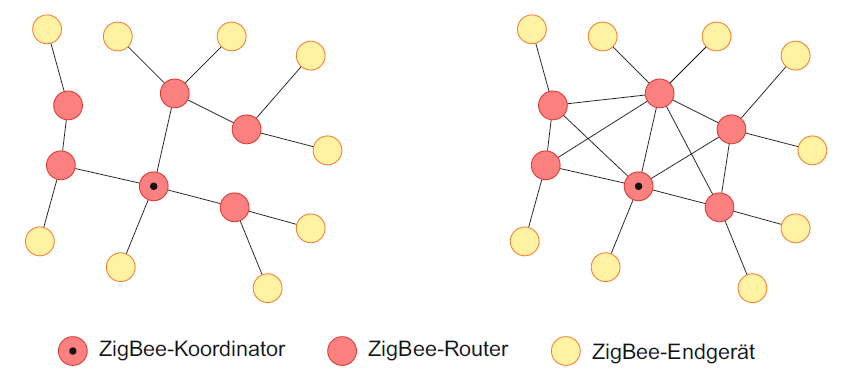
\includegraphics[width=0.8\textwidth]{Zigbee_Netztopologie.png}
	\caption{Zigbee Baum- und Meshnetzwerke \cite[S.~221]{markus_krause_rainer_konrad_zigbee_2014}}	\label{fig:NetzwerktopologienZigbee}
\end{figure}

Wie in der Abbildung \ref{fig:NetzwerktopologienZigbee} bereits angedeutet, kann innerhalb eines Zigbee Meshnetzwerkes zwischen 3 Nodetypen unterschieden werden. Diese besitzen unterschiedliche Aufgaben und Eigenschaften.

\paragraph{Zigbee Koordinator}\label{par:ZigbeeKoordinator}
Als zentrale Einheit übernimmt der \textit{Zigbee Koordinator} Aufgaben wie den Start und die Verwaltung eines PAN (Personal Area Network) inkl. der Definition der wichtigsten Parameter wie der PAN-ID, der Sicherheitsschlüssel sowie die Wahl des IEEE Channels.
In einem Zigbee-Netzwerk gibt es genau ein Gerät das die Rolle des \textit{Zigbee Koordinators} übernimmt. Wenn dieses Gerät das Netzwerk verlässt oder kurzzeitig ausser Betrieb ist, kann das Netzwerk trotzdem weiter bestehen und funktioniert normal weiter.
Jeder \textit{Zigbee-Koordinator} hat gleichzeitig auch die Rolle eines \textit{Zigbee-Router}.

\paragraph{Zigbee Router}\label{par:ZigbeeRouter}
\textit{Zigbee-Router} bilden das eigentliche Meshnetzwerk. Sie übernehmen die Aufgabe des Routings was die Wegentdeckung sowie Weiterleitung von Paketen beinhaltet. Jeder \textit{Zigbee-Router} führt eine Routing-Table welche fortlaufend aktualisiert wird.

\paragraph{Zigbee End-Device}\label{par:ZigbeeEndDevice}
Die einfachste Rolle ist jene des \textit{Zigbee End-Devices}. Sie stehen in einer Parent-Child Beziehung mit einem \textit{Zigbee-Router}.
Diese Kommunikation findet entweder periodisch oder ausgelöst durch einen Userinput statt.
Ankommende Pakete werden jeweils vom Parent-Node gespeichert bis das  \textit{Zigbee End-Devices} diese abruft.
\textit{Zigbee End-Devices} besitzen ausserdem keine Routing Funktionen und gelten deshalb als sehr energiesparend.
Ausgeführt als Sleepy-End-Device können CPU und RAM des entsprechenden Nodes ganz oder teilweise heruntergefahren werden und durch periodische Interrupts geweckt werden.
Dadurch können sehr lange Batteriestandzeiten erreicht werden. \cite{markus_krause_rainer_konrad_zigbee_2014}


\subsection{Zigbee Protokoll Stack}\label{subsec:ZigbeeProtokollStack}
\todo[inline]{Erläuterung des Protokoll Stacks. Möglichst viel Grafiken und nur so viel als nötig Prosa.}

Die Architektur des Zigbee Stacks besteht aus vier Layern, dem Physical layer (PHY), dem MAC layer, dem Network layer (NWK) und dem Application layer (APL).
Abbildung \ref{fig:ArchitekturdesZigbeeProtokollStacks} zeigt den Aufbau des Protokoll Stacks im Detail.
Jede der Schichten ist mit bestimmten Aufgaben betraut und stellt der darüber liegenden Schicht Daten und Dienste bereit.
Nachfolgend wird auf die vier Schichten des Zigbee Stacks eingegangen und deren Funktion und Funktionsweise kurz erläutert.

\begin{figure}[h]
	\centering
	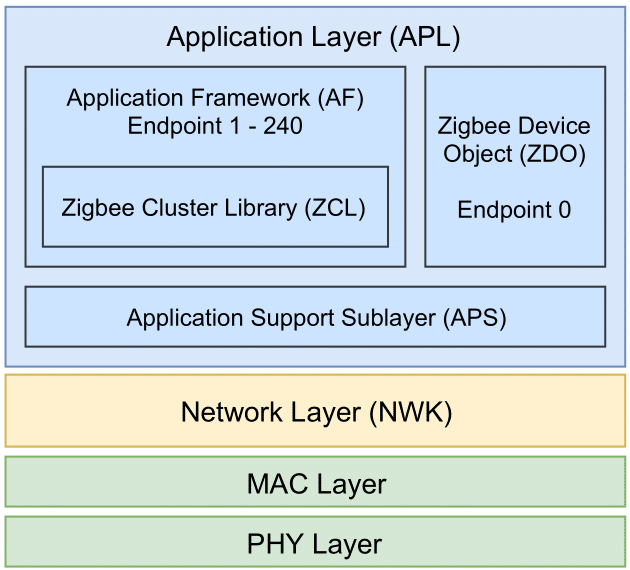
\includegraphics[width=0.7\textwidth]{Zigbee_Architektur.png}
	\caption{Architektur des Zigbee Protokoll Stacks}
	\label{fig:ArchitekturdesZigbeeProtokollStacks}
\end{figure}

\subsubsection{MAC und PHY Layer}\label{subsubsec:MACundPHYLayer}
MAC und PHY Layer werden im Zigbee Protokoll Stack gebildet durch den IEEE 802.15.4 Standard für \textit{Wireless Personal Area Networks (WPAN)}.
Während beispielsweise Wifi oder Bluetooth, welche auf dem selben 2.4 GHz ISM-Funkfrequenzband betrieben werden können, für hohe Datenübertragungsraten konzipiert wurden, ist dieser Standard für kleinere Datenmengen optimiert.
Durch die Vermeidung von unnötigen Steuerinformationen, kann der IEEE 802.15.4 Standard auf einfachster Hardware realisiert und mit kleinstem Energieaufwand betrieben werden.
Ideal also für sogenannte \textit{Wireless Sensor Networks (WSN)} wie beispielsweise Zigbee. \cite{markus_krause_rainer_konrad_ieee_2014}


\subsubsection{Network Layer}\label{subsubsec:Network Layer}
Der Network Layer ist im Zigbee Stack verantwortlich für den Aufbau sowie das Management der Netzwerkfunktionen und das Routing innerhalb dieses Netzwerkes.

\paragraph{Netzaufbau und Adressierung}\label{par:ZigbeeNetzaufbauundAdressierung}
Wie unter \ref{par:ZigbeeKoordinator} bereits erwähnt ist der Koordinator verantwortlich für den Aufbau des Zigbee Netzwerks und der Wahl von entsprechend geeigneten Parametern wie beispielsweise einer 16-Bit PAN-ID oder eines möglichst störungsfreien Funkkanals.
Beim Beitritt eines neuen Funkmoduls wird diesem vom Koordinator eine im Netzwerk einmalige 16-Bit \textit{Short-Address} zugewiesen.
Anhand dieser kann das Funkmodul nun im Netzwerk adressiert werden und es selbst kann damit Routing Funktionen war nehmen.
Die im MAC Layer definierte 64-Bit MAC Adresse kann ebenfalls vollwertig für die Adressierung verwendet werden wobei diese schliesslich in die \textit{Short-Address} übersetzt wird.


\paragraph{Routing}\label{par:Zigbee Routing}
Das Routing geschieht innerhalb von Zigbee Mesh Netzwerken mit dem \textit{ZigBee PRO}-Stackprofil mittels Routingtabellen die jeder Router erstellt und nach führt wenn es Änderungen gibt. In dieser ist die \textit{Short-Address} des Ziels sowie jene des nächsten Hops hinterlegt.
Enthält die Routingtabelle veraltete Einträge oder sind für das entsprechende Ziel noch gar keine Informationen vorhanden, muss ein \textit{Route Discovery} durchgeführt werden.
Hierbei handelt es sich um eine Broadcast Nachricht welche an alle Router gesendet wird. Diese empfangen die Nachricht und leiten sie wiederum als Broadcast an alle Router in Reichweite weiter. Dabei werden die Wegkosten jeweils addiert um diese sobald die Nachricht beim Zielnode angekommen ist, dem Absender mitzuteilen.
Jener Weg mit den geringsten totalen Wegkosten wir so ermittelt und kann schliesslich in der Routingtabelle abgelegt werden.


\subsubsection{Application Support Sublayer (APS)}\label{subsubsec:ApplicationSupportSublayer}


\subsubsection{Application Layer}\label{subsubsec:ZigbeeApplicationLayer}

\paragraph{Zigbee Cluster Library (ZCL)}\label{par:ZigbeeClusterLibrary}

\paragraph{Endpunkte}\label{par:ZigbeeEndpunkte}


\subsubsection{Sicherheit}\label{subsucsec:ZigbeeSicherheit}



\subsection{Zigbee Software Development Kit}\label{subsec:ZigbeeSoftwareDevelopmentKit}
\todo[inline]{Eingesetzte SDK und deren Aufbau beschreiben. Allenfalls die wichtigsten API Funktionen genauer erläutern.}

nRF5 SDK for Thread and Zigbee

ZBOSS stack v3.3.0

Kooperatives Multitasking in ZBOSS

revision 22 of the Zigbee Core Specification.
 
 \begin{figure}[h]
	\centering
	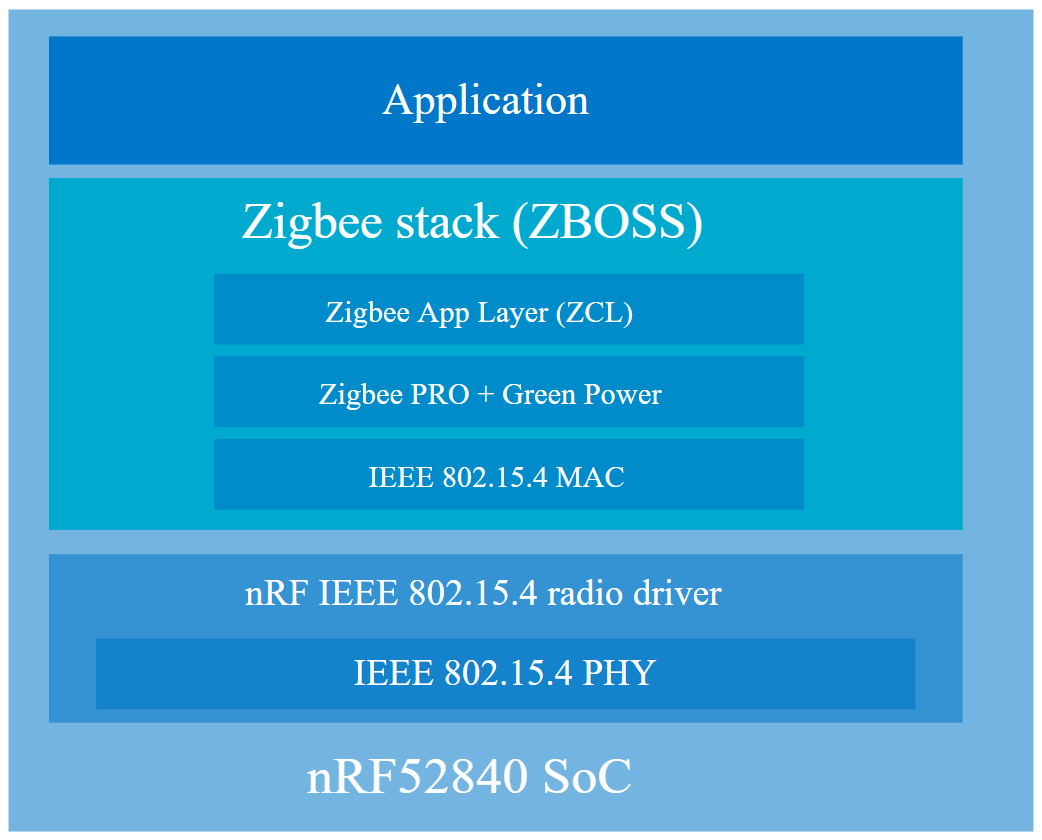
\includegraphics[width=0.6\textwidth]{Zigbee_SDK_Plattform_Design.png}
	\caption{nRF5 SDK for Thread and Zigbee Plattform Design Referenz \cite{nordic_semi_nrf_sdk_for_thread_and_zigbee_2020}}
	\label{fig:ZigbeePlattformDesign}
\end{figure}
 